\documentclass[12pt]{article}

\usepackage[margin=1in]{geometry}
\usepackage{setspace}
\onehalfspacing
\usepackage{amsmath,amssymb,amsthm,mathtools,bm}
\usepackage{booktabs,graphicx,array,multirow}
\usepackage[round,authoryear]{natbib}
\usepackage[hidelinks]{hyperref}
\usepackage{enumitem}
\usepackage{xcolor}
\usepackage{microtype}

\graphicspath{{figures/}}
\setlength{\emergencystretch}{2em}
\setlist{nosep}

\theoremstyle{plain}
\newtheorem{theorem}{Theorem}[section]
\newtheorem{proposition}[theorem]{Proposition}
\newtheorem{corollary}[theorem]{Corollary}
\newtheorem{lemma}[theorem]{Lemma}
\theoremstyle{definition}
\newtheorem{assumption}[theorem]{Assumption}
\newtheorem{definition}[theorem]{Definition}
\theoremstyle{remark}
\newtheorem{remark}[theorem]{Remark}

\DeclareMathOperator{\E}{\mathbb{E}}
\DeclareMathOperator{\Prob}{\mathbb{P}}
\DeclareMathOperator{\Var}{\operatorname{Var}}
\DeclareMathOperator{\Corr}{\operatorname{Corr}}
\DeclareMathOperator*{\argmin}{arg\,min}
\newcommand{\cX}{\mathcal{X}}
\newcommand{\cS}{\mathcal{S}}
\newcommand{\cA}{\mathcal{A}}
\newcommand{\cD}{\mathcal{D}}
\newcommand{\cF}{\mathcal{F}}
\newcommand{\R}{\mathbb{R}}
\newcommand{\x}{\bm{x}}
\newcommand{\etaHat}{\widehat{\eta}}
\newcommand{\etaStar}{\eta^{\star}}
\newcommand{\atlas}{\mathcal{A}_{n_0}}

\title{\textbf{Transferable Structural Proposal Atlases for\\
High-Dimensional Chance-Constrained Simulation Optimization}}
\author{Authors omitted for review}
\date{}

\begin{document}
\maketitle

\begin{abstract}
High-dimensional simulation optimization is statistically impossible under a
tiny target budget without reusable structure.  We study chance-constrained
problems in which source tasks are available before a new target task is
opened.  We propose a dimension-equivariant structural proposal atlas: source
outcomes rank normalized low-frequency policy profiles, target-label-free
profiles provide universal support, and a maximin rule selects a small target
initial design.  The atlas is frozen before target outcomes and can be paired
with any online optimizer.  We prove that unconditional finite-budget coverage
is impossible, give a conditional source-to-target coverage theorem whose
geometry is independent of nominal dimension, and add an optimizer-independent
terminal verifier with a familywise deployment-error bound.  In three held-out
synthetic domains at dimension 1,000, the atlas yields independently certified
feasible recommendations in 60 of 60 trials with three different backends,
whereas common Sobol initial designs yield at most one.  At dimension 10,000 it
certifies all 30 trials across budgets from 10 to 40 target search calls.  An
external electricity-storage holdout confirms an advantage over equal-total-
cost unstructured search, but not over a natural low-frequency grid.  The
results identify transferable structural coverage, rather than a particular
Bayesian-optimization backend, as the main source of sample efficiency.
\end{abstract}

\medskip
\noindent\textbf{Keywords:} simulation optimization; chance constraints;
transfer learning; high-dimensional Bayesian optimization; independent
verification; structural priors

\section{Introduction}\label{sec:introduction}

Simulation optimization is often most valuable precisely where function
evaluation is slow, noisy, and safety constrained.  A policy may contain
hundreds or thousands of coordinated controls, while only a handful of target
simulations are affordable.  Examples include reserve schedules, multi-node
inventory rules, and resource-allocation profiles.  In these settings, the
central statistical difficulty precedes the choice of an acquisition
function: an unstructured initial design has negligible probability of
intersecting a small feasible basin.  A sophisticated sequential optimizer
cannot improve a basin it never observes.

Historical tasks create a possible escape from this difficulty.  Related
systems may have been optimized in earlier markets, networks, or operating
regimes.  Their observations can reveal policy shapes that repeatedly balance
objective quality and chance feasibility.  Yet reusing those observations is
delicate.  Raw coordinates may change dimension, the meaning of individual
controls may not align across tasks, and a target-specific hand-coded anchor
would turn transfer into hidden oracle information.  Moreover, an attractive
recommendation and a deployment-safe recommendation are different statistical
objects.  Reusing the same observations for search and final certification can
make the apparent evaluation budget and the safety claim both misleading.

This paper treats those issues as one information-design problem.  Before a
target task is opened, source outcomes are used to construct a small
\emph{structural proposal atlas}: a set of normalized policy profiles that is
defined in a dimension-equivariant low-frequency coordinate.  Source profiles
are ranked by objective and chance-margin evidence, target-label-free profiles
provide universal structural support, and a maximin rule fills a fixed initial
design.  The atlas is then frozen.  Any target optimizer can consume it; in the
primary implementation we use the standard sparse axis-aligned subspace
Bayesian optimizer (SAASBO).  After search, a separate verifier receives fresh
samples from a frozen, ordered shortlist and never returns those samples to the
optimizer.

The separation is substantive rather than cosmetic.  It lets us ask three
distinct questions.  Does the transferred frontend reach a feasible basin?
Does online optimization improve objective quality once coverage is
established?  Can the final recommendation be independently certified?  It
also forces a transparent cost accounting: source simulation, target search,
and terminal verification are reported separately.

Our contributions are as follows.

\begin{enumerate}[label=(\roman*)]
\item We introduce a target-label-free, dimension-equivariant risk-objective
proposal atlas.  Its low-frequency coordinate has fixed dimension even when
the raw policy dimension changes, and its source-monotone extension is
fail-closed when source directions disagree.

\item We establish the relevant theoretical boundary.  No proper finite atlas
can cover every possible held-out feasible set.  Under an explicit
source-to-target support condition, coordinate error bound, margin regularity,
and safe-depth condition, however, the atlas contains a feasible policy.  The
sufficient condition depends on coordinate geometry rather than nominal policy
dimension.  These and the terminal verification results are machine checked in
Lean 4 without unproved placeholders.

\item We design an optimizer-independent verifier with familywise control of
unsafe deployment and an objective switch guard.  Search, objective-comparison,
and safety-verification samples are tracked separately, so a target search
budget is never reported as a total simulation budget.

\item We perform a causal frontend/backend evaluation.  At dimension 1,000,
the frozen atlas produces true-feasible and independently certified
recommendations in all 60 trials with proposal-only, stacked-GP, and canonical
SAASBO backends.  Matched common-Sobol frontends produce zero, one, and zero,
respectively.  At dimension 10,000, all 30 trials are certified across target
search budgets from 10 to 40 calls.  An electricity-storage holdout confirms a
large total-cost advantage over unstructured Sobol, while a post-confirmatory
structured control shows no advantage over an obvious low-frequency grid.

\item We retain negative findings that delimit the contribution.  Canonical
SAASBO is a replaceable backend rather than a novel algorithm.  A cumulative
heteroscedastic variance model recovers variance shape much better than pooled
variance but does not improve optimization outcomes, so it is reported as a
calibration diagnostic rather than a second headline contribution.
\end{enumerate}

The resulting claim is deliberately narrower than ``solving arbitrary
10,000-dimensional optimization in ten evaluations.''  The method succeeds
when related tasks share a stable, low-dimensional structural coordinate; the
paper states, audits, and stress-tests that condition.  Section
\ref{sec:literature} positions the work.  Sections \ref{sec:problem}--
\ref{sec:theory} give the information contract, atlas, and guarantees.
Sections \ref{sec:experiments} and \ref{sec:results} present the experiments,
and Section \ref{sec:discussion} discusses limits and operational use.

\section{Related Literature}\label{sec:literature}

\paragraph{Simulation optimization and noisy constraints.}
Simulation optimization studies expensive stochastic systems for which
objectives or constraints are available only through simulation
\citep{Fu2002,AmaranEtAl2016}.  Stochastic kriging explicitly separates
response uncertainty from simulation noise \citep{AnkenmanNelsonStaum2010},
while constrained Bayesian optimization models noisy objective and feasibility
observations jointly \citep{LethamEtAl2019}.  Our question occurs one stage
earlier: before fitting a target surrogate, which few ordered profiles should
receive the first simulations?

\paragraph{High-dimensional and functional optimization.}
Trust-region methods and sparse axis-aligned priors can make Bayesian
optimization more robust in large ambient spaces
\citep{ErikssonEtAl2019,ErikssonPoloczek2021,ErikssonJankowiak2021}.  They do
not by themselves encode that coordinates discretize one ordered function.
Functional Bayesian optimization instead searches over function-valued
decisions \citep{VienEtAl2018}.  Our profile coordinate is less flexible but
fully finite: it maps irregular or refined grids into a common cosine summary,
then selects from a declared structural library.  Nominal grid dimension and
effective profile complexity are therefore reported separately.

\paragraph{Transfer and historical-task priors.}
Few-shot deep kernels, hierarchical Gaussian-process priors, source ensembles,
and meta-learned acquisitions transfer different objects across tasks
\citep{WistubaGrabocka2021,RothfussEtAl2021,RothfussEtAl2023,
WangEtAl2024HyperBO,TighineanuEtAl2022,VolppEtAl2020,PanEtAl2024}.
Related work also learns a search space from earlier hyperparameter tasks
\citep{PerroneEtAl2019} or transfers optimizer rankings
\citep{FeurerEtAl2018}.  In contrast, our source archive scores a fixed public
library; it does not learn a target surrogate, acquisition function, or hidden
target-specific representation.  This narrower object makes source cost and
the source-free structural counterfactual directly auditable.  We nevertheless
compare eight native end-to-end transfer pipelines using the same source
information and target budget.

\paragraph{Selection and independent verification.}
Chance-constrained ranking-and-selection procedures allocate simulation to
identify a feasible best system while controlling selection error
\citep{HongLuoNelson2015}.  Post-optimization ranking and selection can also
``clean up'' candidate solutions generated by a heuristic search
\citep{BoeselNelsonKim2003}.  We adopt this separation literally.  Search
produces an ordered shortlist; fresh Bernoulli feasibility replications test
its members; and Bonferroni spending composes candidate-wise exact tests.  The
all-success rule is conservative, so we report power and verification cost in
addition to false certificates.  This differs from treating a surrogate's
posterior feasibility probability as a deployment certificate.

\paragraph{Positioning.}
Without restrictions on the objective and feasible set, no finite
target-label-free design can dominate all others, a point consistent with
no-free-lunch results \citep{WolpertMacready1997}.  Our contribution is not a
distribution-free optimizer.  It is a task-law-conditional experimental-design
protocol for ordered profiles, accompanied by source-free structured controls,
adverse regimes, a negative external control, and explicit cost accounting.

\section{Problem Setting and Available Information}\label{sec:problem}

\subsection{Ordered policy profiles}

Let $h:[0,1]\to[0,1]$ denote an ordered policy profile.  A task $q$ supplies
ordered nodes
\[
  0<t_{q,1}<\cdots<t_{q,d_q}<1
\]
and an integer implementation scale $L_q$.  The deployed vector is
\[
  x_{q,i}(h)=\operatorname{round}\{L_qh(t_{q,i})\},
  \qquad i=1,\ldots,d_q.
\]
Thus $d_q$ is a grid resolution, not by itself the intrinsic dimension of the
admissible profile class.  Regular grids use
$t_{q,i}=(i-1/2)/d_q$; irregular grids are allowed when their ordering is
declared.  A schema may additionally declare channel order.  No claim is made
for an unordered vector with unknown coordinate semantics.

One simulator replication at $x$ returns an objective observation $Y^f_q(x)$
and a scalar constraint observation $Y^g_q(x)$.  We minimize
\[
  f_q(x)=\E[Y^f_q(x)]
\]
subject to the chance constraint
\begin{equation}\label{eq:chance-constraint}
  p_q(x):=\Prob\{Y^g_q(x)\le \tau_q\}\ge 1-\alpha_q.
\end{equation}
The true feasible set is $\cF_q=\{x:p_q(x)\ge1-\alpha_q\}$.
In synthetic experiments, the experimenter reveals truth only after design,
search, shortlisting, and verification are complete, and uses it only to score
the finished decision.

\subsection{Source and target information}

Let $q_1,\ldots,q_m$ be source tasks and $q_\star$ a target task.  Before the
target opens, every source task evaluates the same finite normalized profile
library $\cL=\{h_1,\ldots,h_J\}$.  For each pair $(q,h)$, the source archive
contains $R$ ordinary replications of $(Y^f_q,Y^g_q)$.  The primary method uses
$m=2$, $J=64$, and $R=3$, hence
\begin{equation}\label{eq:source-cost}
  S=mJR=384
\end{equation}
source simulator calls.  The library is constructed without source or target
outcomes; source data only determine which members are selected.

The source archive is supplied before the target problem opens.  In the
synthetic stress test its tasks come from the same declared regime as the
target; in the external study they obey the stated region-holdout rule.  The
method ranks profiles within this archive.  Choosing or purchasing related
historical tasks from a larger repository is a separate upstream decision.

Before target search, the method may use the target's ordered grid, integer
bounds, nominal dimension, and, in declared-schema experiments, channel order.
It may not use a target outcome, feasibility label, noise parameter, optimum,
safe-basin center, or verification sample.  The primary source aggregation is
domain blind: source tasks receive equal weight.  Descriptor-conditioned
weighting is evaluated only as a control.

\subsection{Decision stages and costs}

The initial-design step selects $n_0$ target policies.  A target optimizer may
then use a total of $N\ge n_0$ search calls and return an ordered list of at
most $K_s$ distinct candidates.  This list and its order are fixed before
fresh verification simulations begin.  The final outcome is either a
certified deployment or abstention.

We report the costs
\begin{equation}\label{eq:cost-identity}
  C_{\rm all}=S+N+V,
  \qquad
  C_{\rm amort}(M)=\frac{S}{M}+N+V,
\end{equation}
where $V$ is the realized independent-verification cost and $M$ is the number
of target deployments sharing one source archive.  ``Equal preverification
cost'' means that $S+N$ is matched before $V$; it is not called equal total
cost.

\subsection{Endpoints}

The primary search endpoint is whether the $N$ target evaluations contain a
truly feasible policy.  The primary deployment endpoint is whether the
verifier returns a truly feasible policy.  We also report false certificates,
verification calls, and a penalized loss that retains failures in the
denominator.  Conditional regret is reported only when a feasible policy
exists and is not used alone to compare methods with different feasible
counts.  A separate fixed library defines synthetic regret and an unattainable
finite-library upper bound; neither affects an implementable decision.

\section{Dimension-Equivariant Structural Proposal Atlas}\label{sec:atlas}

\subsection{Low-Frequency Policy Coordinate}

Write $z_i=x_i/L_q\in[0,1]$ for the normalized policy.  The raw policy length
changes across tasks, so direct coordinate-wise transfer is not well defined.
For a fixed frequency cap $K$, define
\begin{align}
 \bar z &= d^{-1}\sum_{i=0}^{d-1}z_i,\qquad
 s_z=\left[d^{-1}\sum_{i=0}^{d-1}(z_i-\bar z)^2\right]^{1/2},\label{eq:dc}\\
 c_k(z)&=\frac{2}{d}\sum_{i=0}^{d-1}(z_i-\bar z)
 \cos\left(\frac{\pi k(i+1/2)}{d}\right),\quad k=1,\ldots,K.\label{eq:dct}
\end{align}
The implemented coordinate $\etaHat_d(\x)$ contains $\bar z$, $s_z$, and a
frequency-penalized selection of the coefficients in
\eqref{eq:dct}, followed by a fixed diagonal quadratic expansion.  We use
$K\le 8$.  Its dimension depends on $K$, not on $d$.  The cosine basis also
admits an inverse map: a coordinate is reconstructed as a constant profile plus
the selected modes, clipped to $[0,1]$, and rounded to the target integer
bounds.

This coordinate encodes a specific structural hypothesis: slowly varying
policy profiles and their coarse shape transfer more reliably than the identity
of a raw coordinate.  It does not assert that every high-dimensional problem
is low frequency.  Domain- and dimension-holdout experiments test whether this
hypothesis remains useful.

\subsection{Universal Support and Source Templates}

The candidate library is the union of two components.  The \emph{universal
structural support} contains target-label-free constant, monotone, and
low-frequency profiles generated from $(d,L_q)$ alone.  It supplies coverage
when source outcomes are misleading or do not include a useful endpoint.  The
\emph{source templates} are normalized profiles observed in every source task.

For each source task, replicated observations estimate an objective score and
a chance-margin score.  Scores are converted to within-task percentiles before
aggregation, avoiding a common numerical scale assumption across domains.
Profiles that are robustly source feasible are preferred.  Candidate templates
on the source objective--risk Pareto frontier are selected under five fixed
scalarizations: risk-only, objective-only, and three intermediate weights.
This ranking uses observed source data only.  It never uses a source analytic
optimizer or a target outcome.

After the extreme Pareto templates are included, the remaining slots are
filled by a maximin rule in $\etaHat$: at each step we select the candidate
whose minimum coordinate distance to the current atlas is largest, with fixed
penalties for source risk and objective rank.  The result is a deterministic
risk-objective atlas of size at most $n_0$.

\subsection{Fail-Closed Source-Monotone Envelope}

A final source-only extension tests whether the zero-frequency coefficient
$\bar z$ has a common chance-margin direction.  For each source task $q'$, let
$\rho_{q'}$ be the rank correlation between $\bar z$ and observed chance
margin.  With threshold $\kappa=0.25$, the upper constant endpoint is admitted
only if at least two source tasks all satisfy $\rho_{q'}\le-\kappa$; the lower
endpoint is admitted only if all satisfy $\rho_{q'}\ge\kappa$.  Admission
replaces an existing slot, so the budget remains $n_0$.  If neither condition
holds, the update is the identity.

The original three synthetic domains reject this extension in all 60 primary
cells, making the final version exactly equal to the base atlas there.  The
electricity family admits it using source markets before the confirmatory
market is opened.  Source agreement is evidence for a transferable direction,
not proof that the target shares it; Section \ref{sec:theory} states the
additional target monotonicity condition explicitly.

\subsection{Training and Deployment Algorithm}

The full frontend is summarized below.

\begin{enumerate}[label=\textbf{A\arabic*.},leftmargin=3.2em]
\item Normalize the 64 shared profiles in each source task and compute
replication-based objective and chance-margin summaries.
\item Convert summaries to within-source percentile ranks; retain robust
source-feasible Pareto templates under the fixed risk-objective weights.
\item Form the candidate union of source templates and universal structural
support; map all candidates into $\etaHat_d$.
\item Seed the atlas with selected Pareto extremes and fill remaining slots by
the penalized maximin rule.
\item Apply the fail-closed source-monotone endpoint test without changing
atlas size.
\item Freeze the atlas before the first target simulation.  Evaluate its
$n_0$ policies, then pass the observations to the chosen online backend.
\end{enumerate}

The proposal is learned offline but is not free: its 384 source simulations
are included in archive-fair and total-cost comparisons.  When the same archive
is reused for many targets, this cost may be amortized operationally; our
tables do not assume such amortization.

\section{Coverage and Verification Guarantees}\label{sec:theory}

This section separates three claims that are often conflated: a finite
proposal cannot cover arbitrary targets; it can cover targets satisfying a
structural transfer condition; and a recommendation can be verified without
assuming the search model is correct.  Complete machine-checked statements are
mapped to the implementation in Appendix \ref{app:lean}.

\subsection{Why an Explicit Transfer Condition Is Necessary}

\begin{theorem}[Finite-atlas no-free-lunch]\label{thm:nfl}
Let $\cX$ be finite and let $\cA\subsetneq\cX$ be any proper proposal atlas
frozen before target labels.  There exists a nonempty feasible set
$\cF\subseteq\cX$ such that $\cA\cap\cF=\varnothing$.
\end{theorem}

\begin{proof}
Choose $x_0\in\cX\setminus\cA$ and set $\cF=\{x_0\}$.  Then $\cF$ is
nonempty and is missed by $\cA$.
\end{proof}

Theorem \ref{thm:nfl} is elementary but decisive.  Neither source learning nor
a nonlinear encoder can guarantee that ten target-label-free proposals hit an
arbitrary feasible set.  A positive result must identify what transfers.

\subsection{Aligned Geometric Atlas Coverage}

Let $\etaStar$ be an ideal transferable coordinate and $\etaHat$ the coordinate
learned from source information.  Let $\cS$ be the finite source-support
library and $\atlas\subseteq\cS$ the selected atlas.  Distances below are in
the common coordinate space.

\begin{assumption}[Atlas coverage]\label{ass:atlas-cover}
For every $s\in\cS$, there is $a\in\atlas$ such that
$\|\etaHat(s)-\etaHat(a)\|\le r_{\mathrm{cover}}$, with
$|\atlas|\le n_0$.
\end{assumption}

\begin{assumption}[Coordinate approximation]\label{ass:coordinate}
For each relevant policy $x$,
$\|\etaHat(x)-\etaStar(x)\|\le\epsilon_\eta$.
\end{assumption}

\begin{assumption}[Source-target support]\label{ass:support}
There exists a target-safe center $x_c$ and a source-support policy
$s_c\in\cS$ such that
$\|\etaStar(x_c)-\etaStar(s_c)\|\le\Delta_{\mathrm{task}}$.
\end{assumption}

\begin{assumption}[One-sided margin regularity and safe depth]
\label{ass:margin}
The target chance margin satisfies
\begin{equation}\label{eq:lipschitz}
 m_q(x)\le m_q(y)+L_m\|\etaHat(x)-\etaHat(y)\|
\end{equation}
for relevant $x,y$, and $m_q(x_c)+\gamma\le0$ for some $\gamma>0$.
\end{assumption}

\begin{theorem}[Aligned finite-atlas coverage]\label{thm:coverage}
Under Assumptions \ref{ass:atlas-cover}--\ref{ass:margin}, if
\begin{equation}\label{eq:coverage-condition}
 L_m\bigl(r_{\mathrm{cover}}+\Delta_{\mathrm{task}}
       +2\epsilon_\eta\bigr)\le\gamma,
\end{equation}
then at least one $a\in\atlas$ is feasible for the target task.
\end{theorem}

\begin{proof}
Assumptions \ref{ass:coordinate} and \ref{ass:support}, followed by the
triangle inequality, place $s_c$ within
$\Delta_{\mathrm{task}}+2\epsilon_\eta$ of $x_c$ in the learned coordinate.
Assumption \ref{ass:atlas-cover} supplies $a\in\atlas$ at an additional
distance at most $r_{\mathrm{cover}}$.  By \eqref{eq:lipschitz} and
\eqref{eq:coverage-condition},
\[
 m_q(a)\le m_q(x_c)+L_m(r_{\mathrm{cover}}+Delta_{\mathrm{task}}
 +2\epsilon_\eta)\le -\gamma+\gamma=0.
\]
Thus $a$ is feasible.
\end{proof}

\begin{corollary}[Nominal-dimension independence]\label{cor:dimension}
If $r_{\mathrm{cover}}$, $\Delta_{\mathrm{task}}$, $\epsilon_\eta$, $L_m$,
and $\gamma$ remain controlled as $d$ changes, the sufficient condition
\eqref{eq:coverage-condition} does not depend on $d$.
\end{corollary}

Corollary \ref{cor:dimension} is a conditional effective-dimension result, not
an assertion that the constants are automatically stable.  The finite-library
post-run audit verifies positive slack in all three synthetic domains (Table
\ref{tab:coverage-audit}) under registered library quantities.  It does not
certify a global Lipschitz constant for every policy, so the global theorem
remains an explicit modeling condition.

\begin{table}[t]
\centering
\caption{Post-run finite-library coverage audit.  Slack is safe radius minus
the audited atlas/support radius.  These diagnostics were not used for target
selection.}
\label{tab:coverage-audit}
\begin{tabular}{lrrrr}
\toprule
Domain & $r_{cover}$ & Support shift & Safe radius & Slack \\
\midrule
FactorShock & 0.0502 & 0.0000 & 0.3277 & 0.2775 \\
Inventory & 0.0307 & 0.0000 & 0.1322 & 0.1015 \\
Queue & 0.0384 & 0.0019 & 0.1298 & 0.0895 \\
\bottomrule
\end{tabular}

\end{table}

\subsection{Fail-Closed Monotone Extension}

Let $U$ and $L$ denote the upper and lower normalized constant policies.  The
source-monotone test of Section \ref{sec:atlas} either replaces one atlas entry
with an admitted endpoint or returns the base atlas unchanged.

\begin{proposition}[Fail-closed identity and budget]\label{prop:failclosed}
If neither source direction satisfies the admission threshold, the extension
returns the base atlas exactly.  In all cases its cardinality is at most $n_0$.
\end{proposition}

\begin{proposition}[Transferred endpoint safety]\label{prop:endpoint}
Suppose all source tasks admit $U$, the target margin is nonincreasing in the
zero-frequency coordinate, and $U$ is coordinate-wise maximal.  If any target
policy is feasible, then $U$ is feasible.  A symmetric statement holds for
the admitted lower endpoint and a nondecreasing target margin.
\end{proposition}

\begin{proof}
For a feasible witness $x_s$, maximality gives
$\bar z(x_s)\le\bar z(U)$.  Target monotonicity gives
$m_q(U)\le m_q(x_s)\le0$.  The lower-endpoint case reverses the order.
\end{proof}

The source rank statistic is only the admission rule.  Target monotonicity is
the additional identifiability condition and is not inferred by logic alone.

\subsection{Optimizer-Independent Terminal Verification}

After search, the backend freezes an ordered shortlist of at most three
policies: an objective challenger, the backend recommendation, and a
safe-interior support policy.  Candidate $j$ is tested with fresh samples and
error allocation $\delta_j$.  Let $E_j$ be the event that candidate $j$ is
certified even though it is unsafe.

\begin{theorem}[Ordered-shortlist safety]\label{thm:verifier}
If $\Prob(E_j)\le\delta_j$ for every frozen candidate, then the probability
that the first certified shortlist member is unsafe is at most
$\sum_j\delta_j$.
\end{theorem}

\begin{proof}
Unsafe deployment implies $E_j$ for at least one candidate that could be
selected.  The union bound yields the result; no property of the optimizer is
used.
\end{proof}

The challenger can replace a certified incumbent only if a one-sided upper
confidence bound on their paired objective difference is negative.  Let
$\delta_{\mathrm{obj}}$ bound failure of that objective upper bound.

\begin{corollary}[Joint deployment and switch bound]\label{cor:joint}
If $\sum_j\delta_j\le\delta_{\mathrm{safe}}$, then the probability of unsafe
deployment or an incorrect objective switch is at most
$\delta_{\mathrm{safe}}+\delta_{\mathrm{obj}}$.
\end{corollary}

The implementation spends familywise error $0.05$ across the frozen shortlist
and uses eight fresh paired objective replications per compared policy when an
objective switch is attempted.  Verification samples never update the search
posterior.

For the external energy experiment, one verification replication is a fresh
calendar window and success means satisfying the reliability requirement in
that window.  If $K\sim\mathrm{Binomial}(n,p)$, the probability of $n$ successes
is $p^n$.

\begin{proposition}[Exact all-success certificate]\label{prop:binomial}
For any infeasible reliability probability $p\le p_{\mathrm{req}}$,
\begin{equation}
 \Prob_p(K=n)=p^n\le p_{\mathrm{req}}^n.
\end{equation}
Error spending over a frozen finite shortlist gives the corresponding
familywise bound.
\end{proposition}

The registered first stage uses 80 independent windows.  At the 0.95 required
probability and registered confidence level, the one-sided Clopper--Pearson
rule certifies only the all-success count; the implementation equivalence is
regression tested and Proposition \ref{prop:binomial} is machine checked from
the binomial law.

\subsection{Optional Cumulative Heteroscedastic Calibration}

Some simulation tasks provide observable local exposures $A(x)$ and shared
shock exposures $N(x)$.  The optional cumulative factor model is
\begin{equation}\label{eq:hvd}
 v_C(x)=A(x)^\top\Lambda A(x)+N(x)^\top B N(x)
       +N(x)^\top\omega+v_0,
\end{equation}
with nonnegative diagonal $\Lambda$, positive-semidefinite $B$, and projected
nonnegative linear/floor terms.  This decomposition recovers local,
shared-shock, linear, and floor contributions and is used only in the HVD
diagnostic.  The primary atlas and verifier do not require it.  The distinction
matters because better variance fit is not the same as better optimization;
Section \ref{sec:hvd-results} reports both outcomes.

\section{Experimental Design}\label{sec:experiments}

\subsection{Evaluation Questions}

The experiment matrix is organized around five preregistered questions.

\begin{enumerate}[label=Q\arabic*.]
\item Does the frozen atlas, rather than the online backend, cause feasible-
basin coverage?
\item Are both universal support and source templates needed?
\item How does the method compare with transfer methods receiving the same
source archive and target budget, and with target-only methods receiving the
same total search cost?
\item Does performance persist as raw dimension and the ratio $d/N$ increase?
\item Does the structural coordinate transfer to a held-out real-data control
problem, and what happens against an obvious structured control?
\end{enumerate}

A sixth diagnostic asks whether cumulative factor-HVD improves variance fit or
operational optimization.  It was governed by a promotion rule requiring both
calibration improvement and at least one operational gain without harm.

\subsection{Synthetic Task Family}

We use three chance-constrained policy families.  Each policy has integer
entries in $\{0,\ldots,100\}$, giving $101^d$ raw alternatives.

\begin{description}[leftmargin=1.2em,style=nextline]
\item[FactorShock.] The objective and constraint depend on coarse policy level,
tail level, and dispersion.  Constraint noise contains three local exposures
(level gap, tail gap, and spread) and two correlated shared-shock exposures
(oscillation and tail shock), with the exact cumulative form in
\eqref{eq:hvd}.

\item[Inventory.] The policy is divided into stock, reorder, and safety-stock
blocks.  The objective balances holding, backlog, reorder, and safety losses;
the chance constraint represents service reliability.  Local variance
exposures are backlog, holding, and stockout, while demand level and demand
volatility are shared shocks.

\item[Queue.] The policy is divided into capacity, priority, and smoothing
blocks.  The objective balances waiting and resource costs, and the chance
constraint defines a safe operating pocket.  Local exposures are queue, wait,
and utilization; shared exposures are arrival bursts and common load.
\end{description}

These are not arbitrary high-dimensional functions.  They deliberately embed
different operations mechanisms in normalized, low-dimensional policy
summaries and heteroscedastic noise.  Their role is to test whether a
dimension-equivariant profile learned from two mechanisms transfers to the
third.  In each leave-one-domain-out fold, the other two domains form the
source archive.  Each target domain uses 20 independent simulation seeds
(80--99) at $d=1000$ and fixed registered geometry.  Truth is evaluated only
post-run.  The extreme-dimension study uses ten seeds per domain at $d=10000$.

\subsection{External Electricity-Storage Holdout}

The external study uses hourly load, forecast, and price series from Open Power
System Data \citep{OPSD2020}.  A $d=1000$ integer profile controls storage
reserve and state-of-charge behavior.  The simulator includes charge and
discharge limits, round-trip efficiency, reserve floor, cycling cost, spill,
and unserved-energy penalties.  The chance constraint limits the fraction of
unserved demand windows.

The source markets are Austria 2017 and Denmark DK1 2017.  Denmark DK2 2018 is
the development target.  Great Britain 2018 is opened once as the untouched
20-seed confirmatory target.  The source-monotone endpoint rule is decided
before Great Britain outcomes.  Search, audit, and verification use separated
calendar samples.  We compare the frozen atlas at $N=13$ with (i) a natural
constant-policy low-frequency grid at $N=13$, added as a post-confirmatory
fairness audit, and (ii) common Sobol with $N=397$, equal to 384 source plus 13
target-search calls.

\subsection{Methods and Fairness Contracts}

The frontend/backend factorial uses two initial designs: the frozen atlas and
common Sobol.  Each is paired with proposal-only selection, a stacked transfer
GP, and canonical SAASBO.  Canonical means a BoTorch
\texttt{SaasFullyBayesianSingleTaskGP} refit at every adaptive iteration
\citep{BalandatEtAl2020,ErikssonJankowiak2021}; periodic-capped SAAS appears
only as a separately named target-only computational control.

Archive-fair transfer comparisons receive the same 384 source calls, frozen
$n_0=10$ initial design, target seeds, $N=13$ target-search calls, and terminal
verifier.  They include Safe F-PACOH, RGPE, stacked GP, transfer multi-task GP,
FSBO, HyperBO, MetaBO, and MALIBO.  Official code paths are used with documented
compatibility adaptations to the scalar constrained interface.  Target-only
TuRBO, SCBO, and periodic-capped SAAS receive $N=397$ target-search calls, equal
to the final method's source-plus-target search cost.  All final comparisons
use the same independent verifier.

The frontend component ablation retrains and regenerates every proposal from
the same source archive.  It compares universal support only, source templates
only, and their combined maximin atlas.  This is the supported structural
ablation.  Earlier orthogonality, sparsity, additive, manifold, transformer,
KG, and Thompson-sampling variants remain development diagnostics and are not
recast as coequal contributions.

\subsection{Verification, Metrics, and Inference}

The synthetic verifier uses an ordered three-policy shortlist with candidate
budgets 80, 128, and 128, familywise error 0.05, and a fresh paired objective
guard when switching incumbents.  It may stop after the first candidate.
Consequently, verification calls are variable and are reported as a cost,
not normalized away.  The energy verifier uses 80 fresh windows in its first
stage and the exact binomial/Clopper--Pearson rule in Proposition
\ref{prop:binomial}.

We report true-feasible recommendations, independently certified
recommendations, false certificates, feasible regret conditional on true
feasibility, and verification cost.  Post-run HVD diagnostics report
log-variance RMSE and variance-shape correlation over a fixed audit set.  The
statistical plan uses paired seeds, 10,000-sample bootstrap intervals for
median paired differences, exact McNemar tests for paired binary outcomes,
Wilcoxon signed-rank tests for paired continuous outcomes, and Holm adjustment
within preregistered confirmatory families.  Domain strata are descriptive
heterogeneity analyses, not separate confirmatory families.  Failed and timed-
out runs remain in the immutable registry; all release-required cells used
below are complete.

\section{Results}\label{sec:results}

\subsection{The Frontend Determines Feasible-Basin Coverage}

Table \ref{tab:frontend-backend} gives the main causal comparison.  With the
frozen atlas, all three backends produce true-feasible and independently
certified recommendations in all 60 domain-seed pairs, with no false
certificate.  Replacing only the frontend by common Sobol reduces these counts
to 0/60 for proposal-only, 1/60 for stacked GP, and 0/60 for canonical SAASBO.
For the preregistered proposal-only and SAAS comparisons, the Holm-adjusted
McNemar $p$-value is $6.94\times10^{-18}$ for both feasibility and
certification.  Figure \ref{fig:frontend-backend} shows the aggregate contrast.

\begin{table}[t]
\centering
\small
\caption{Frontend/backend factorial at $d=1000$.  Frozen-atlas arms use
$n_0=10$ and at most three adaptive calls; proposal-only stops at ten.  Every
arm uses the same independent verifier.}
\label{tab:frontend-backend}
\resizebox{\textwidth}{!}{\begin{tabular}{lllrrrr}
\toprule
Domain & Frontend & Backend & Feasible & Certified & False & Med. regret \\
\midrule
FactorShock & Frozen atlas & Proposal only & 20/20 & 20/20 & 0 & 0.0082 \\
FactorShock & Frozen atlas & Stacked GP & 20/20 & 20/20 & 0 & 0.0082 \\
FactorShock & Frozen atlas & Canonical SAASBO & 20/20 & 20/20 & 0 & 0.0082 \\
FactorShock & Common Sobol & Proposal only & 0/20 & 0/20 & 0 & -- \\
FactorShock & Common Sobol & Stacked GP & 0/20 & 0/20 & 0 & -- \\
FactorShock & Common Sobol & Canonical SAASBO & 0/20 & 0/20 & 0 & -- \\
\midrule
Inventory & Frozen atlas & Proposal only & 20/20 & 20/20 & 0 & 0.0116 \\
Inventory & Frozen atlas & Stacked GP & 20/20 & 20/20 & 0 & 0.0116 \\
Inventory & Frozen atlas & Canonical SAASBO & 20/20 & 20/20 & 0 & 0.0031 \\
Inventory & Common Sobol & Proposal only & 0/20 & 0/20 & 0 & -- \\
Inventory & Common Sobol & Stacked GP & 1/20 & 1/20 & 0 & 0.0108 \\
Inventory & Common Sobol & Canonical SAASBO & 0/20 & 0/20 & 0 & -- \\
\midrule
Queue & Frozen atlas & Proposal only & 20/20 & 20/20 & 0 & 0.0029 \\
Queue & Frozen atlas & Stacked GP & 20/20 & 20/20 & 0 & 0.0029 \\
Queue & Frozen atlas & Canonical SAASBO & 20/20 & 20/20 & 0 & 0.0015 \\
Queue & Common Sobol & Proposal only & 0/20 & 0/20 & 0 & -- \\
Queue & Common Sobol & Stacked GP & 0/20 & 0/20 & 0 & -- \\
Queue & Common Sobol & Canonical SAASBO & 0/20 & 0/20 & 0 & -- \\
\bottomrule
\end{tabular}
}
\end{table}

\begin{figure}[t]
\centering
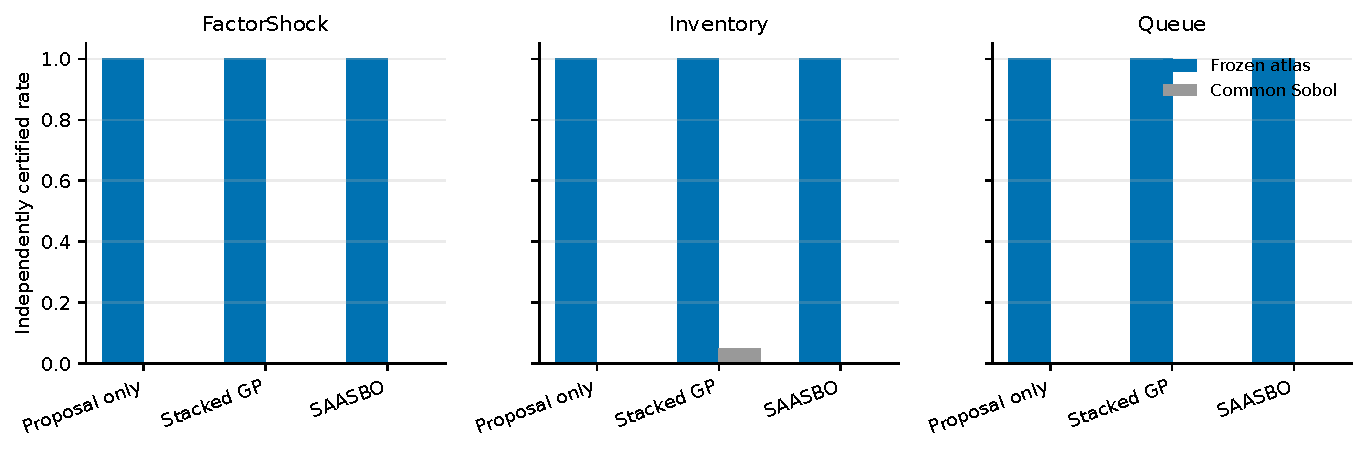
\includegraphics[width=0.82\textwidth]{frontend_backend.pdf}
\caption{Feasible-basin coverage is driven by the frozen structural frontend,
not by the backend.  Counts aggregate 20 seeds in each of three domains.}
\label{fig:frontend-backend}
\end{figure}

Once coverage is established, the backend affects objective quality.  Across
all 60 frozen-atlas pairs, canonical SAASBO improves regret over proposal-only
in 29 seeds, loses in two, and ties in 29; the Holm-adjusted Wilcoxon
$p$-value is $1.16\times10^{-6}$.  It improves over stacked GP in 29 seeds,
loses in three, and ties in 28 ($p_{\mathrm{Holm}}=1.49\times10^{-6}$).
The median paired difference is zero because FactorShock and many other pairs
tie, while Inventory and Queue contain the improvements.  The target-stage
convergence paths in Figure \ref{fig:convergence} make the decomposition clear:
the initial atlas reaches the feasible region, and the three adaptive calls
occasionally improve its objective.

\begin{figure}[t]
\centering
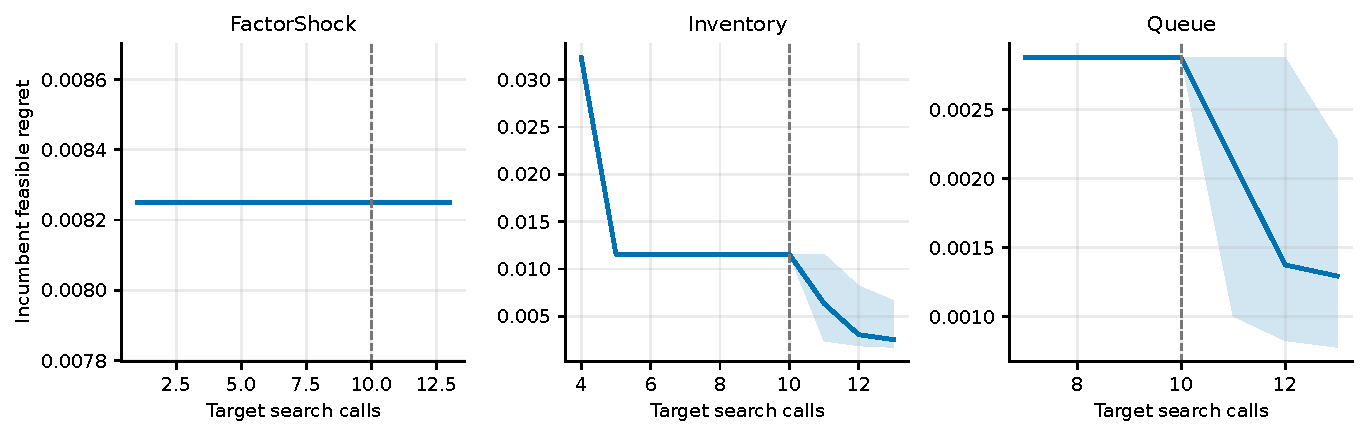
\includegraphics[width=0.86\textwidth]{target_convergence.pdf}
\caption{Median best true-feasible objective gap during target search.  Missing
early values mean that no evaluated point was truly feasible at that call.
Verification samples are excluded.}
\label{fig:convergence}
\end{figure}

\subsection{Both Atlas Components Matter}

Universal structural support alone reaches 27/60 feasible trials; source
templates alone reach 40/60; their combined maximin atlas reaches 60/60
(Table \ref{tab:components} and Figure \ref{fig:components}).  Universal
support is particularly important as a source-misspecification fallback,
whereas source templates concentrate probability mass around empirically safe,
low-cost profiles.  The combined atlas is therefore not merely the best source
profile copied to a new dimension.

\begin{table}[t]
\centering
\caption{Causal frontend component ablation with the same source archive,
target seeds, proposal budget, and verifier.}
\label{tab:components}
\begin{tabular}{lrrrr}
\toprule
Frontend component & Feasible & Certified & False & Med. regret \\
\midrule
Universal support & 27/60 & 23/60 & 0 & 0.0082 \\
Source templates & 40/60 & 40/60 & 0 & 0.0072 \\
Combined maximin atlas & 60/60 & 60/60 & 0 & 0.0082 \\
\bottomrule
\end{tabular}

\end{table}

\begin{figure}[t]
\centering
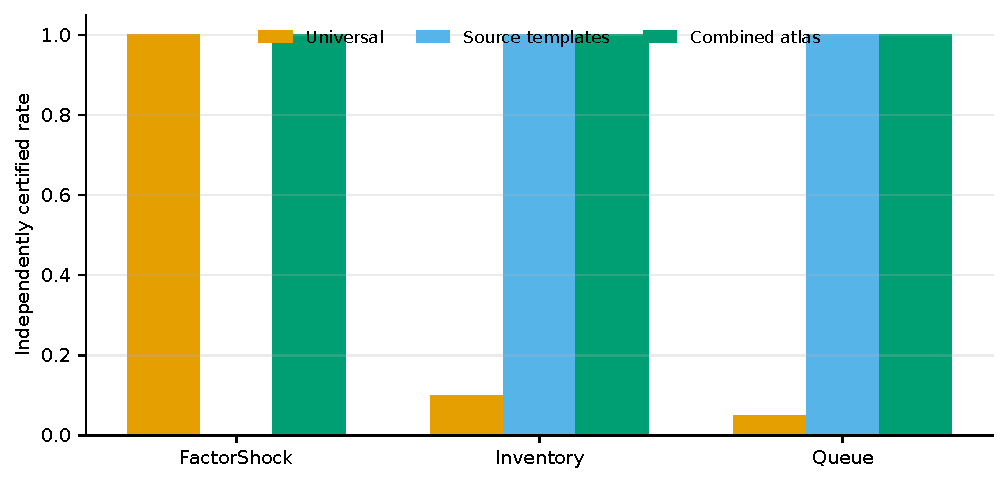
\includegraphics[width=0.70\textwidth]{frontend_components.pdf}
\caption{Feasible and independently certified recommendations under the
frontend component ablation.}
\label{fig:components}
\end{figure}

\subsection{Archive-Fair Transfer and Total-Cost Controls}

Table \ref{tab:transfer} compares transfer methods under exactly the same
source archive, frozen initial design, target budget, seeds, and verifier.
Because every method receives the strong atlas, most achieve high feasible
coverage.  Safe F-PACOH reaches 56/60, RGPE and FSBO 59/60, transfer MTGP
57/60, and stacked GP, HyperBO, MetaBO, MALIBO, and canonical SAASBO 60/60.
Canonical SAASBO has the lowest aggregate median feasible regret (0.0038),
whereas the other displayed methods have 0.0082.  Verification cost differs
materially, demonstrating why the 60/60 coverage count alone is insufficient.

\begin{table}[t]
\centering
\small
\caption{Archive-fair transfer comparison at $d=1000$, $S=384$, $n_0=10$,
and $N=13$.  Mean verification includes safety and any fresh objective-
comparison calls.}
\label{tab:transfer}
\begin{tabular}{lrrrrr}
\toprule
Method & Feasible & Certified & False & Med. regret & Mean verify \\
\midrule
Atlas + canonical SAASBO & 60/60 & 60/60 & 0 & 0.0038 & 173.9 \\
Safe F-PACOH & 56/60 & 56/60 & 0 & 0.0082 & 215.5 \\
RGPE & 59/60 & 59/60 & 0 & 0.0082 & 154.9 \\
Stacked GP & 60/60 & 60/60 & 0 & 0.0082 & 90.9 \\
Transfer MTGP & 57/60 & 57/60 & 0 & 0.0082 & 204.3 \\
FSBO & 59/60 & 59/60 & 0 & 0.0082 & 181.6 \\
HyperBO & 60/60 & 60/60 & 0 & 0.0082 & 211.7 \\
MetaBO & 60/60 & 60/60 & 0 & 0.0082 & 158.9 \\
MALIBO & 60/60 & 60/60 & 0 & 0.0082 & 162.9 \\
\bottomrule
\end{tabular}

\end{table}

The equal-total-search-cost comparison is more severe.  Target-only TuRBO and
SCBO receive 397 target-search calls and find no feasible recommendation in 60
trials.  Periodic-capped target-only SAAS finds two, both certified.  The atlas
plus canonical SAASBO uses 384 source calls and 13 target-search calls and
certifies all 60 (Table \ref{tab:totalcost}).  The Holm-adjusted McNemar
$p$-values for the final method versus each target-only control are below
$3\times10^{-17}$.  These results support reuse of related source simulations;
they do not imply that source calls are free or that the frontend is uniformly
better than every task-specific structured design.

\begin{table}[t]
\centering
\caption{Equal source-plus-search-cost comparison.  Verification is applied
after search and reported separately.  ``Target-only SAASBO'' denotes the
audited periodic-capped control, not canonical every-iteration SAASBO.}
\label{tab:totalcost}
\begin{tabular}{lrrrrr}
\toprule
Method & Source & Search & Feasible & Certified & False \\
\midrule
Atlas + canonical SAASBO & 384 & 13 & 60/60 & 60/60 & 0 \\
Target-only TuRBO & 0 & 397 & 0/60 & 0/60 & 0 \\
Target-only SCBO & 0 & 397 & 0/60 & 0/60 & 0 \\
Target-only SAASBO & 0 & 397 & 2/60 & 2/60 & 0 \\
\bottomrule
\end{tabular}

\end{table}

\subsection{Dimension and Target-Budget Frontier}

At $d=1000$, proposal-only at ten search calls and canonical SAASBO at 13 both
certify all 60 trials; aggregate median regret improves from 0.00825 to 0.00383.
At $d=10000$, all 30 trials are feasible and certified with zero false
certificates at search budgets 10, 13, 20, and 40 (Table
\ref{tab:dimension}).  The corresponding $d/N$ ratios range from 1,000 to 250.
Median regret is 0.00825, 0.00825, 0.00451, and 0.00579.  The deterioration
from $N=20$ to $N=40$ is retained rather than smoothed away; additional
adaptive search is not monotonically beneficial under this finite stochastic
protocol.

\begin{table}[t]
\centering
\small
\caption{Dimension and target-search budget.  Source archive size remains
384; verification is additional and variable.}
\label{tab:dimension}
\begin{tabular}{rrrrrrrr}
\toprule
$d$ & Search & $d/N$ & Source & Feasible & Certified & False & Med. regret \\
\midrule
1000 & 10 & 100.0 & 384 & 60/60 & 60/60 & 0 & 0.0082 \\
1000 & 13 & 76.9 & 384 & 60/60 & 60/60 & 0 & 0.0038 \\
10000 & 10 & 1000.0 & 384 & 30/30 & 30/30 & 0 & 0.0082 \\
10000 & 13 & 769.2 & 384 & 30/30 & 30/30 & 0 & 0.0082 \\
10000 & 20 & 500.0 & 384 & 30/30 & 30/30 & 0 & 0.0045 \\
10000 & 40 & 250.0 & 384 & 30/30 & 30/30 & 0 & 0.0058 \\
\bottomrule
\end{tabular}

\end{table}

\begin{figure}[t]
\centering
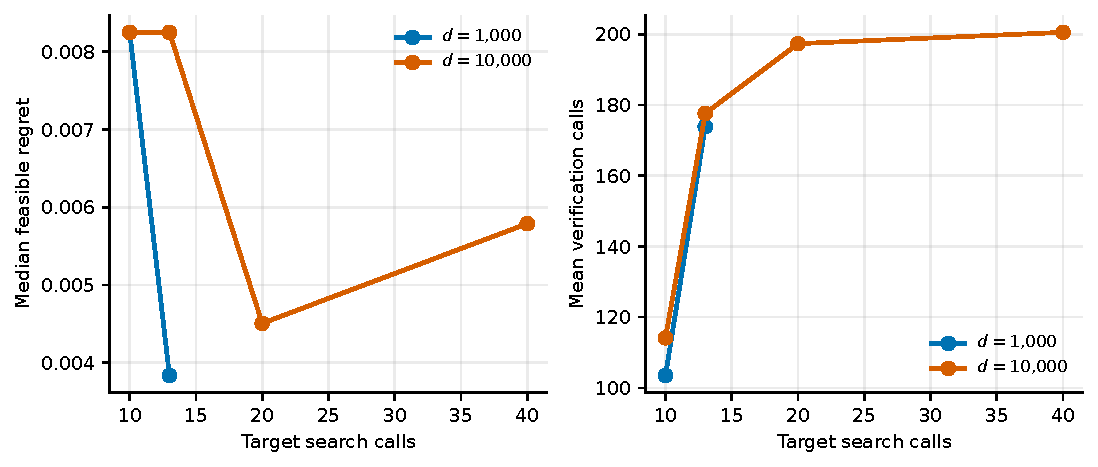
\includegraphics[width=0.90\textwidth]{dimension_budget.pdf}
\caption{Dimension/budget frontier: aggregate median feasible regret (left)
and mean verification calls (right).  The $d=10000$ result is an effective-
dimension stress test under the registered structural family.}
\label{fig:dimension}
\end{figure}

The result is consistent with Corollary \ref{cor:dimension}: the raw dimension
can grow while the profile coordinate remains fixed.  It is not evidence that
SAASBO or the atlas can identify an arbitrary sparse set of raw coordinates in
ten calls.  Indeed, the common-Sobol negative controls show that the same
backend without structural coverage fails at $d=1000$.

\subsection{External Electricity Holdout}\label{sec:energy-results}

All three energy arms are independently certified in 20/20 seeds with no false
certificate (Table \ref{tab:energy}).  The frozen atlas at $N=13$ beats
equal-total-cost common Sobol at $N=397$ in all 20 paired seeds.  The median
objective difference (atlas minus Sobol) is $-0.05331$, with bootstrap 95\%
interval $[-0.05408,-0.05058]$ and one-sided exact sign
$p=9.54\times10^{-7}$.

The natural low-frequency grid changes the interpretation.  The atlas wins
9/20 and loses 11/20; the median difference is $0.000945$, with 95\% interval
$[-0.00108,0.00180]$ and one-sided sign $p=0.748$.  Thus the external result
supports low-frequency structural compression and a large advantage over
unstructured total-cost search.  It does not establish that source learning
outperforms an obvious domain-specific low-frequency control.

\begin{table}[t]
\centering
\caption{Untouched Great Britain electricity-storage holdout and retained
post-confirmatory fairness controls.}
\label{tab:energy}
\begin{tabular}{lrrrr}
\toprule
Arm & Certified & False & Median objective & Mean verify \\
\midrule
Frozen atlas, $N=13$ & 20/20 & 0 & 0.0976 & 80.0 \\
Natural low-frequency grid, $N=13$ & 20/20 & 0 & 0.0956 & 80.0 \\
Common Sobol, $N=397$ & 20/20 & 0 & 0.1488 & 80.0 \\
\bottomrule
\end{tabular}

\end{table}

\begin{figure}[t]
\centering
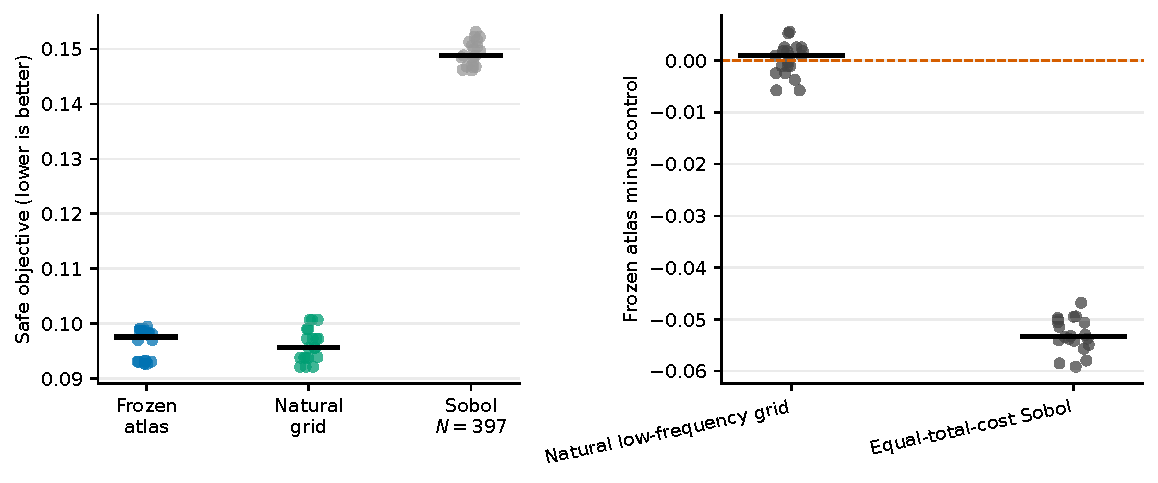
\includegraphics[width=0.90\textwidth]{external_energy.pdf}
\caption{External energy paired differences.  Negative values favor the
frozen atlas.  The left panel is a retained negative result; the right panel
is the equal-total-cost unstructured control.}
\label{fig:energy}
\end{figure}

\subsection{Heteroscedastic Decomposition Is a Calibration Diagnostic}
\label{sec:hvd-results}

The cumulative factor model sharply improves variance-shape recovery under a
matched proposal, canonical SCBO backend, verifier, and 20-seed design.  Mean
log-variance RMSE falls from 1.158 to 0.219 in FactorShock, 0.577 to 0.349 in
Inventory, and 0.501 to 0.254 in Queue.  Shape correlation rises from zero
under pooled variance to 0.919, 0.953, and 0.995.  The Holm-adjusted Wilcoxon
$p$-value is $1.14\times10^{-10}$ for both log-RMSE and shape correlation.

Operationally, however, both models produce 59/60 feasible and certified
recommendations, zero false certificates, and identical median paired regret.
The HVD model also increases mean verification cost in Inventory and Queue.
It therefore fails the preregistered promotion rule and remains an optional
risk-calibration diagnostic.

\begin{table}[t]
\centering
\small
\caption{Pooled versus cumulative factor-HVD.  Variance diagnostics are
post-run only; they do not enter target selection.}
\label{tab:hvd}
\begin{tabular}{lllrrrr}
\toprule
Domain & Variance model & Feasible & Log-RMSE & Shape corr. & Mean verify \\
\midrule
FactorShock & Pooled & 20/20 & 1.158 & 0.000 & 159.2 \\
FactorShock & Cumulative factor-HVD & 20/20 & 0.219 & 0.919 & 158.4 \\
\midrule
Inventory & Pooled & 20/20 & 0.577 & 0.000 & 182.4 \\
Inventory & Cumulative factor-HVD & 20/20 & 0.349 & 0.953 & 184.0 \\
\midrule
Queue & Pooled & 19/20 & 0.501 & 0.000 & 190.4 \\
Queue & Cumulative factor-HVD & 19/20 & 0.254 & 0.995 & 197.6 \\
\bottomrule
\end{tabular}

\end{table}

\begin{figure}[t]
\centering
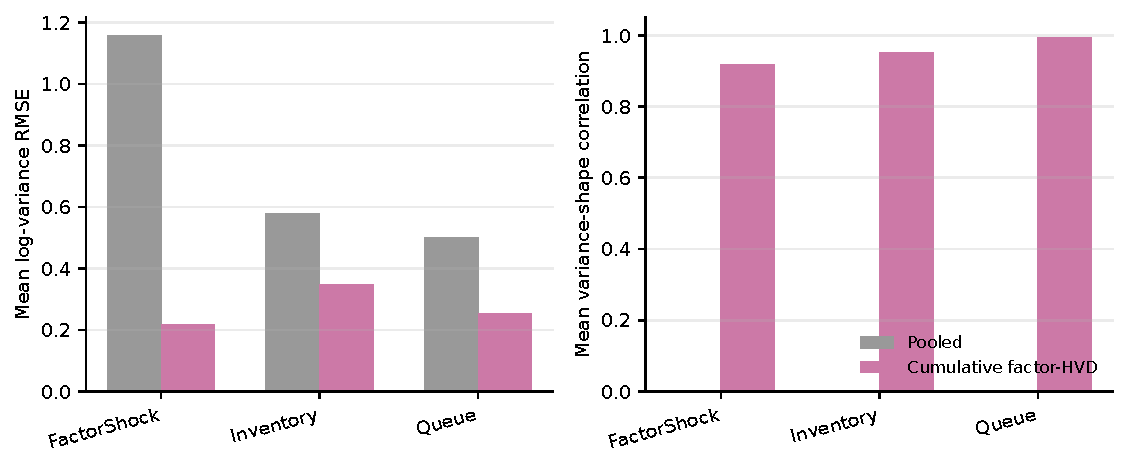
\includegraphics[width=0.78\textwidth]{hvd_diagnostic.pdf}
\caption{Cumulative factor-HVD recovers variance shape but does not improve
feasible recovery or regret in the matched causal experiment.}
\label{fig:hvd}
\end{figure}

\section{Discussion}\label{sec:discussion}

\subsection{What the evidence supports}

Source outcomes help when source and target tasks organize safety around
similar policy shapes.  That is the central empirical claim, and the adverse
regimes make it testable rather than automatic.  Source scoring improves
coverage on the full randomized mixture, but the regime table and Energy
study show concrete cases in which it loses.

This interpretation differs from claiming a generic high-dimensional
optimizer.  The raw vector may contain $10^4$ coordinates, but the decision is
an ordered profile and the library has finite structural complexity.  A
controller may still require a fine lookup table, so profile-grid refinement
is operationally relevant.  It is not equivalent to adding $10^4$ unrelated
decision variables.  The proper benefit is invariance to representation
resolution under shared profile structure.

\subsection{What Energy teaches us}

The Energy reversal shows that a generic structural design can beat source
scoring when rankings from held-out regions do not transfer.  Because V3 was
fixed before its outcomes, changing the score now would turn a test case into
development data.  We keep the result as a negative control and as a practical
boundary on when the method should be used.

The practical implication is a diagnostic choice.  If historical tasks and a
new target share an ordered policy semantics and source rank stability can be
validated on genuinely held-out tasks, source scoring is reasonable.  If the
target is temporally or geographically shifted and generic low-frequency
structure already has a credible physical basis, the generic maximin design is
the safer default.  The method should abstain from a transfer claim when these
conditions cannot be assessed.

The current method begins after this assessment: a source archive has already
been supplied, and the algorithm ranks profiles inside it.  It does not
retrieve related tasks from an unrestricted historical database.  Regime-matched
synthetic sources therefore identify the value of scoring a relevant archive,
whereas Energy shows the cost of archive mismatch.  Source retrieval and its
own data-acquisition cost remain separate research and operational decisions.

\subsection{When the source archive pays for itself}

Ten target calls do not beat 394 target calls for a single target.  The source
archive becomes economically plausible only when it is reused.  Let
$C_0=N_0+V_0$ be the expected target-only calls per deployment and
$C_A=N_A+V_A$ the source-design calls excluding the archive.  The call-count
break-even number of deployments is
\begin{equation}\label{eq:break-even}
 M_{\rm break}=\left\lceil\frac{S}{C_0-C_A}\right\rceil,
 \qquad C_0>C_A.
\end{equation}
In the randomized primary experiment, mean-call estimates give thresholds of
about 7, 9, and 11 targets relative to generic DCT, natural structure, and raw
Sobol.  This arithmetic does not include differences in simulator setup,
wall-clock parallelism, or policy quality, and Energy shows that paying the
archive can still be inferior.  It is a planning threshold, not a dominance
theorem.

Table \ref{tab:outcome-adjusted-cost} also reports calls per certified
deployment, but that ratio is only a descriptive planning aid.  A complete
operational comparison would attach decision-maker costs to unsafe deployment,
abstention, and objective quality.  We report those components separately
rather than choose their relative value on the reader's behalf.

\subsection{Search and verification answer different questions}

Independent verification frequently costs an order of magnitude more than
target search because it answers a different question.  Search asks whether a
promising policy has been found.  Verification asks whether a fixed policy can
be deployed with a specified false-certification bound.  A target-only
optimizer making the same safety claim must also pay for fresh samples.

The all-success rule is valid but weak near the threshold, which explains why
feasible coverage exceeds certified deployment.  Future studies should fix a
more efficient exact or sequential test in advance and use block-aware
verification when temporal replications are not iid.

\subsection{Benchmark fit and remaining threats}

Fixing the generator before confirmatory runs reduces development overfitting
but cannot erase it: the task law, library, and stress axes were created within
the project.  Ordered semantics are a strong prior.  Energy covers only five
regions, and the native transfer study has only three historical families.
The archive is assumed to have been supplied; source retrieval is unsolved.
Three replications cannot order near ties, source aggregation can hide task
disagreement, and a finite library can miss the safe region entirely.  Regret
uses a finite evaluation library rather than the unknown continuous optimum,
and one functional-SCBO failure remains in the denominator.  The theory is
conditional on alignment, independence within each regime, and the declared
replication law.  Finally, the same target seeds appear at all three grid
resolutions, so 480-cell totals are descriptive rather than 480 independent
tasks.

\section{Conclusion}\label{sec:conclusion}

High-dimensional chance-constrained simulation optimization cannot be made
sample efficient by acquisition design alone when a tiny target design misses
the feasible region.  We addressed that bottleneck with a source-learned,
dimension-equivariant structural proposal atlas, a replaceable online backend,
and an independent terminal verifier.  The theoretical analysis first rules
out unconditional finite-atlas coverage and then gives an explicit geometric
condition under which coverage is independent of nominal policy dimension.

The experiments identify the atlas as the dominant source of feasible-basin
coverage.  At dimension 1,000 it succeeds across three backends and all 60
trials, while matched common-Sobol designs almost always fail.  Canonical
SAASBO improves objective quality after coverage, but is not essential to
feasibility and is not a methodological contribution.  The dimension-10,000
and external energy studies support transfer of low-frequency structure, with
the important qualification that source learning does not beat an obvious
structured energy control.  Cumulative heteroscedastic decomposition improves
variance calibration but not optimization in the registered causal test.

The broader lesson is that historical simulations should be evaluated as an
experimental-design resource: what policy geometry do they cover, what target
assumption makes that geometry transferable, and how much independent evidence
is required before deployment?  Separating those questions from the optimizer
produces stronger attribution, more honest cost accounting, and a method whose
limits are as explicit as its gains.

\clearpage
\appendix

\section{Finite Algorithm}\label{app:algorithm}

\noindent\fbox{\begin{minipage}{0.94\textwidth}
\textbf{Algorithm 1: Source-scored structural initial design}
\begin{enumerate}[label=\arabic*.]
\item Generate the declared 64-profile outcome-free library on 128 regular
midpoints using seed 20260808.
\item For every source task and profile, compute the replicated objective mean
and the Gaussian chance-margin statistic in \eqref{eq:source-margin}.
\item Convert each statistic to deterministic within-task average-tie
percentile ranks; average the ranks uniformly across source tasks.
\item Compute exact Voronoi-cell cosine coefficients $c_0,\ldots,c_8$, divide
$c_k$ by $1+.25k$, append all nine diagonal squares, and standardize the 18
coordinates over the library.
\item Append source safety and objective ranks.  Select the first center by
\eqref{eq:first-center}; select nine further centers by
\eqref{eq:farthest-first}.
\item Linearly interpolate each selected profile to the declared target grid,
clip to bounds, and deterministically round.  Freeze these ten policies before
the first target outcome.
\item Run any declared target backend.  Freeze a distinct ordered shortlist
before verification.
\item Test each shortlist candidate on its independent all-success stream.
Deploy the first certificate; abstain if none certifies.
\end{enumerate}
\end{minipage}}

The stable tie order is safety rank, objective rank, profile identifier for the
first center and finite-library index for farthest-first.  Robust source
feasibility is diagnostic only.  There is no endpoint replacement, hidden
scalarization, target-outcome repair, or target-oracle branch in a non-oracle
arm.

\section{Additional Statistical Results}\label{app:additional-results}

\subsection{Verifier thresholds}

Table \ref{tab:verifier-power-table} gives exact power calculations.  At
$n=80$, the Clopper--Pearson lower-bound rule equals the all-success rule.  At
$n=160$, its preregistered sensitivity threshold permits two failures.  The
primary results retain the all-success protocol.

\begin{table}[htbp]
\centering
\small
\caption{Exact candidate-wise certificate power at budgets 80 and 160.}
\label{tab:verifier-power-table}
\begin{tabular}{rrrrrr}
\toprule
$n$ & $p$ & All-success power & CP threshold & Allowed failures & CP power \\
\midrule
80 & 0.950 & 0.017 & 80 & 0 & 0.017 \\
80 & 0.975 & 0.132 & 80 & 0 & 0.132 \\
80 & 0.990 & 0.448 & 80 & 0 & 0.448 \\
80 & 0.995 & 0.670 & 80 & 0 & 0.670 \\
80 & 1.000 & 1.000 & 80 & 0 & 1.000 \\
160 & 0.950 & 0.000 & 158 & 2 & 0.012 \\
160 & 0.975 & 0.017 & 158 & 2 & 0.234 \\
160 & 0.990 & 0.200 & 158 & 2 & 0.784 \\
160 & 0.995 & 0.448 & 158 & 2 & 0.953 \\
160 & 1.000 & 1.000 & 158 & 2 & 1.000 \\
\bottomrule
\end{tabular}

\end{table}

\subsection{Full sensitivity matrix}

The full one-factor sensitivity matrix is reported in Table
\ref{tab:sensitivity-full}.  Entries are ordered by the tested levels in the
second column.  Effective-rank levels are explicit overrides; all other rows
include the frozen baseline level.  The nonmonotone responses, the zero
certificate rate at $\alpha=.01$, and the immaterial frequency penalty are
retained rather than optimized away.

\begin{table}[htbp]
\centering
\scriptsize
\caption{One-factor sensitivity of the source-scored design at $d=1000$.
Each rate aggregates eight regimes and 20 independent tasks per regime.}
\label{tab:sensitivity-full}
\resizebox{0.98\textwidth}{!}{\begin{tabular}{llll}
\toprule
Factor & Tested levels & Feasible (\%) & Certified (\%) \\
\midrule
Effective rank & 4/8/16/32 & 89.4/85.0/84.4/83.8 & 55.6/36.3/25.6/29.4 \\
Chance level $\alpha$ & .01/.05/.1 & 95.0/95.0/95.0 & 0.0/46.2/29.4 \\
Calibrated safe mass & .03/.08/.18 & 69.4/95.0/99.4 & 22.5/46.2/70.0 \\
Initial-design size $n_0$ & 5/10/20 & 79.4/95.0/96.9 & 42.5/46.2/46.9 \\
Source tasks & 1/2/4 & 85.0/95.0/95.6 & 33.8/46.2/45.0 \\
Profiles per source task & 32/64/128 & 83.1/95.0/73.8 & 38.1/46.2/38.8 \\
Source replications & 1/3/5 & 92.5/95.0/92.5 & 45.0/46.2/45.6 \\
Retained frequency $K$ & 4/8/16 & 81.9/95.0/95.6 & 43.1/46.2/48.1 \\
Frequency penalty $\kappa$ & 0/.25/1 & 95.0/95.0/95.0 & 46.2/46.2/46.2 \\
Safety-rank weight & .25/1/4 & 95.0/95.0/95.0 & 46.9/46.2/46.2 \\
Objective-rank weight & .25/1/4 & 95.0/95.0/95.0 & 46.9/46.2/46.2 \\
First-center safety weight & .25/.5/.75 & 62.5/95.0/95.0 & 32.5/46.2/45.0 \\
\bottomrule
\end{tabular}
}
\end{table}

Recorded wall time is descriptive rather than a resource-normalized endpoint.
On the mixed CPU cluster, the primary ten-point initial-design arms average
1.2--1.7 seconds per synthetic task, whereas 394-call source-free controls
average about 59 seconds and the 394-call functional-SCBO arm has a median of
about 677 seconds.  The synthetic simulator is analytic and cheap, so these
figures measure implementation overhead rather than the time of a physical
simulator; simulation-call accounting remains the portable comparison.

\subsection{Native end-to-end transfer}

\begin{table}[htbp]
\centering
\small
\caption{Native transfer pipelines at $N=20$ with the same 384-call source
archive and independent verifier.  Each method retains its own initialization
and online adaptation.}
\label{tab:native-transfer}
\resizebox{0.88\textwidth}{!}{\begin{tabular}{lrrrrr}
\toprule
Native method & FactorShock & Inventory & Queue & Total & False \\
\midrule
Safe F-PACOH & 0/20 & 0/20 & 0/20 & 0/60 & 0 \\
RGPE & 14/20 & 16/20 & 0/20 & 30/60 & 0 \\
Stacked GP & 0/20 & 13/20 & 0/20 & 13/60 & 0 \\
MTGP & 1/20 & 0/20 & 0/20 & 1/60 & 0 \\
FSBO & 6/20 & 2/20 & 0/20 & 8/60 & 0 \\
HyperBO & 0/20 & 0/20 & 0/20 & 0/60 & 0 \\
MetaBO & 19/20 & 9/20 & 0/20 & 28/60 & 0 \\
MALIBO & 12/20 & 2/20 & 0/20 & 14/60 & 0 \\
\bottomrule
\end{tabular}
}
\end{table}

No method certifies a Queue task.  These 60-task totals measure repeatability
on three fixed families, not generalization to a population of domains.

\subsection{Energy temporal audit}

\begin{table}[htbp]
\centering
\small
\caption{Postdecision Energy temporal stability.  Counts are descriptive and
do not replace the declared empirical-window certificate.}
\label{tab:temporal-audit}
\begin{tabular}{lrrrr}
\toprule
Matrix & Originally certified & Block stable & Nonoverlap stable & Joint stable \\
\midrule
Energy V2 & 317 & 303/317 & 316/317 & 303/317 \\
Functional V2 & 62 & 59/62 & 61/62 & 58/62 \\
Energy V3 & 358 & 312/358 & 358/358 & 312/358 \\
\bottomrule
\end{tabular}

\end{table}

V3 preserves all 358 original certificates under physically nonoverlapping
windows but 312 under the joint block criterion.  Shared calendars and only
five regions preclude an iid market-population interpretation.

\section{Secondary Cumulative-Variance Diagnostic}\label{app:hvd}

The project originally studied cumulative heteroscedastic variance
decomposition.  Under matched policies, the factor-HVD model represents local
and shared exposure and improves held-out variance-shape estimation.  Table
\ref{tab:hvd-diagnostic} gives the final matched diagnostic.

\begin{table}[htbp]
\centering
\small
\caption{Pooled variance versus cumulative factor-HVD.  HVD improves
calibration but not feasible recovery or verification cost.}
\label{tab:hvd-diagnostic}
\resizebox{\textwidth}{!}{\begin{tabular}{lllrrrr}
\toprule
Domain & Variance model & Feasible & Log-RMSE & Shape corr. & Mean verify \\
\midrule
FactorShock & Pooled & 20/20 & 1.158 & 0.000 & 159.2 \\
FactorShock & Cumulative factor-HVD & 20/20 & 0.219 & 0.919 & 158.4 \\
\midrule
Inventory & Pooled & 20/20 & 0.577 & 0.000 & 182.4 \\
Inventory & Cumulative factor-HVD & 20/20 & 0.349 & 0.953 & 184.0 \\
\midrule
Queue & Pooled & 19/20 & 0.501 & 0.000 & 190.4 \\
Queue & Cumulative factor-HVD & 19/20 & 0.254 & 0.995 & 197.6 \\
\bottomrule
\end{tabular}
}
\end{table}

Because both variance models recover the same feasible counts and HVD slightly
increases verification cost in Inventory and Queue, HVD is not included in the
paper's claimed optimization method.  Its formal results remain in the proof
archive as reusable mechanistic results.

\section{Machine-Checked Proof Map}\label{app:lean}

The Lean 4 project builds against mathlib without \texttt{sorry},
\texttt{admit}, or project-defined \texttt{axiom}.  Table \ref{tab:lean-map}
maps manuscript claims to their principal files.  Lean proves each displayed
implication; source-target alignment and simulator-distribution assumptions
remain scientific premises.

\begin{table}[htbp]
\centering
\small
\caption{Principal Lean files under \texttt{proof/SCOLHKG/}.}
\label{tab:lean-map}
\begin{tabular}{>{\raggedright\arraybackslash}p{0.39\textwidth}>{\raggedright\arraybackslash}p{0.52\textwidth}}
\toprule
Claim & File \\
\midrule
Finite-atlas no-free-lunch & \texttt{Real/ProposalNoFreeLunch.lean} \\
Profile-coordinate and interpolation error & \texttt{Real/ProfileCoordinateConsistency.lean} \\
Farthest-first factor-two coverage & \texttt{Real/FarthestFirstKCenter.lean} \\
Finite source-mean and rank recovery & \texttt{Measure/SourceRankRecovery.lean}, \texttt{Real/SourceRankRecovery.lean} \\
Task-law coverage calibration & \texttt{Measure/TaskAtlasCoverage.lean} \\
Aligned geometric coverage & \texttt{Real/GeometricAtlasCoverage.lean} \\
Exact all-success candidate validity & \texttt{Measure/ExactBinomialCertificate.lean} \\
Composed frontend and budget interfaces & \texttt{Real/PaperMainline.lean} \\
\bottomrule
\end{tabular}
\end{table}

\section{Reproducibility Contract}\label{app:reproducibility}

The final evidence registry contains 14 matrix contracts, 12 compact analyses,
and SHA-256 commitments for 17,360 result cells.  It records one retained
algorithmic failure and no integrity failure.  Every row identifies the task,
source archive, initial design, method, implementation commit, verifier,
source/search/verification calls, and postdecision truth reconstruction.

Tables and figures in this manuscript are generated only from compact JSON and
CSV analyses.  The renderer does not read checkpoints, pickle files, model
weights, or exported policy vectors.  Runtime artifacts are unnecessary for
auditing the displayed results.  The method specification, randomized task
law, Energy data contract, proof receipt, and rendering manifest are versioned
separately so that a theory version cannot be silently paired with another
experiment version.


\clearpage
\phantomsection
\label{page:references}
\bibliographystyle{plainnat}
\bibliography{references}

\end{document}
